\documentclass[a4paper, 14pt]{extarticle}


% ====== Localization & fonts ======
\usepackage{xcolor}
\usepackage{fontspec}
\usepackage{polyglossia} % Russian lang
\setdefaultlanguage{russian}
\setmainfont{Times New Roman}
\newfontfamily\cyrillicfont{Times New Roman}

% TODO look for better; don't like this one
\setmonofont[Scale=0.9]{DejaVu Sans Mono}
\newfontfamily{\cyrillicfonttt}{DejaVu Sans Mono}[Scale=0.8]

% ====== Math ======
\usepackage{amsmath} % Math stuff
\usepackage{mathtools}
\usepackage{gensymb}
\usepackage{amssymb}

% ====== Other text spacing ======

\usepackage{setspace} % String spacing
\onehalfspacing

\usepackage{parskip} % The red line
\setlength{\parskip}{15pt} % Sep beetween paragraphs

\usepackage{enumitem}
\setlist{nosep, topsep=-10pt} % Remove sep-s beetween list elements

% ====== Source code listings ======

\usepackage{listings} % Source code
\lstset{
	basicstyle=\ttfamily,
	breaklines=true,
	breakatwhitespace=true,
	commentstyle=\color{green},
	keywordstyle=\bfseries\color{blue},
	tabsize=4
}

\lstdefinestyle{num}{
	numbers=left,
	numbersep=0.5cm,
	numberstyle=\ttfamily,
	xleftmargin=0.85cm,
}

\lstdefinestyle{framed_num}{
	frame=single,
	numbers=left,
	numbersep=0.5cm,
	numberstyle=\ttfamily\color{red},
	xleftmargin=1cm,
	framexleftmargin=1cm
}

\lstdefinestyle{sql_style}{
	morekeywords=[10]{while, do, procedure, begin, end, if, tinyint, enum, datetime, boolean, declare, function, return, deterministic, is}
}

\renewcommand{\lstlistingname}{Листинг}

% ====== CSV ======
\usepackage{csvsimple} % Load CSV

% ====== References ======
\usepackage{hyperref} % Links
\hypersetup{
	colorlinks,
	citecolor=black,
	filecolor=black,
	linkcolor=black,
	urlcolor=black
}


% ====== Captions ======
\usepackage{caption}
\usepackage{subcaption}
\captionsetup[figure]{name=Рисунок, labelsep=endash, parskip=0pt}

\captionsetup[lstlisting]{
	labelsep=period,
	justification=RaggedLeft,
	parskip=0pt,
	singlelinecheck=false,
	skip=3pt
}

\captionsetup[table]{
	labelsep=period,
	justification=RaggedLeft,
	parskip=0pt,
	singlelinecheck=false,
	skip=3pt
}

\captionsetup[figure]{
	name=Рисунок,
	justification=centering,
	labelsep=period,
	parskip=6pt,
	skip=3pt
}

% ====== Misc ======
\usepackage{metalogo} % Logos for LaTeX
\usepackage{lipsum} % Lorem ipsum
\usepackage{graphicx} % Pictures
\usepackage{tabularx} % X-tables
\usepackage{csquotes} % French quoutes
\usepackage{multirow}

\usepackage{lastpage}

\usepackage{placeins} % FloatBarrier

\usepackage[final]{pdfpages} % Include PDF
\setboolean{@twoside}{false}

% ====== Plotting ======
\usepackage{tikz}
\usepackage{pgfplots}
\usepackage{pgfplotstable}
\pgfplotsset{compat=newest}
\usepgfplotslibrary{dateplot}


% ====== My commands ======
\newcommand{\addonsubheader}[1]{{\center{\bfseries \vspace{-0.5cm} #1} \\ \vspace{15pt}}}

\newcommand{\definition}[1]{\textbf{#1}}
\newcommand{\screenshot}[3]{
	\begin{figure}[h]
		\centering
		\includegraphics[#1]{#2}
		\caption{#3}
	\end{figure}
}

% ====== Counters ======

\numberwithin{equation}{section}

\newcounter{stepcounter}[subsubsection]

\newcommand\steppar[1][\DefaultOpt]{
	\def\DefaultOpt{#1}
	\paragraph{Шаг №\thestepcounter.}
	\refstepcounter{stepcounter}
}


% ====== Page layout ======
\usepackage[ % Margins
left=1cm,
right=1cm,
top=2cm,
bottom=2cm	
]{geometry}


% ====== Headers ======
\usepackage{fancyhdr}
\pagestyle{fancy}


% ====== Document sectioning ======

\usepackage{titlesec}

\newcommand\sectionbreak{\clearpage} % Each section on a new page

\titlespacing*{\paragraph}{0pt}{15pt}{6pt}
\titlespacing*{\subparagraph}{0pt}{15pt}{3pt}


\begin{document}
	\begin{titlepage}
		{\centering
			{\bfseries
				
\includegraphics[height=8cm]{logo.jpeg}\\
				Unity. Precision. Perfection.\\
				\vspace{3.5cm}
				\uppercase{Конспект лекций} \\
				по дисциплине \enquote{Методы оптимизации}\\
			}
			\vspace{\fill}
		}
		\begin{tabular}{l l}
			\textbf{Лектор}: & Балтрашевич Владимир Эдуардович\\
			\textbf{Страниц}: & \pageref{LastPage}\\
			\textbf{Последнее обновление}: & \today{}\\ 
			\textbf{Автор}: & Корытов Павел, 6304\\
		\end{tabular}
		
		\vspace{2cm}
		{\centering
			Санкт-Петербург \\
			\the\year\\
		}
	\end{titlepage}
	
	\tableofcontents
	\newpage
	\section*{Замечания}
	Используемое ПО:
	\begin{itemize}
		\item \XeLaTeX, дистрибутив TeX Live 2018
		\item Microsoft OneNote
		\item Jupyter Notebook
	\end{itemize}
	Первые две лекции включены как pdf из OneNote.\\
	(MAYBE) TODO: переписать с использованием \TeX. 
	
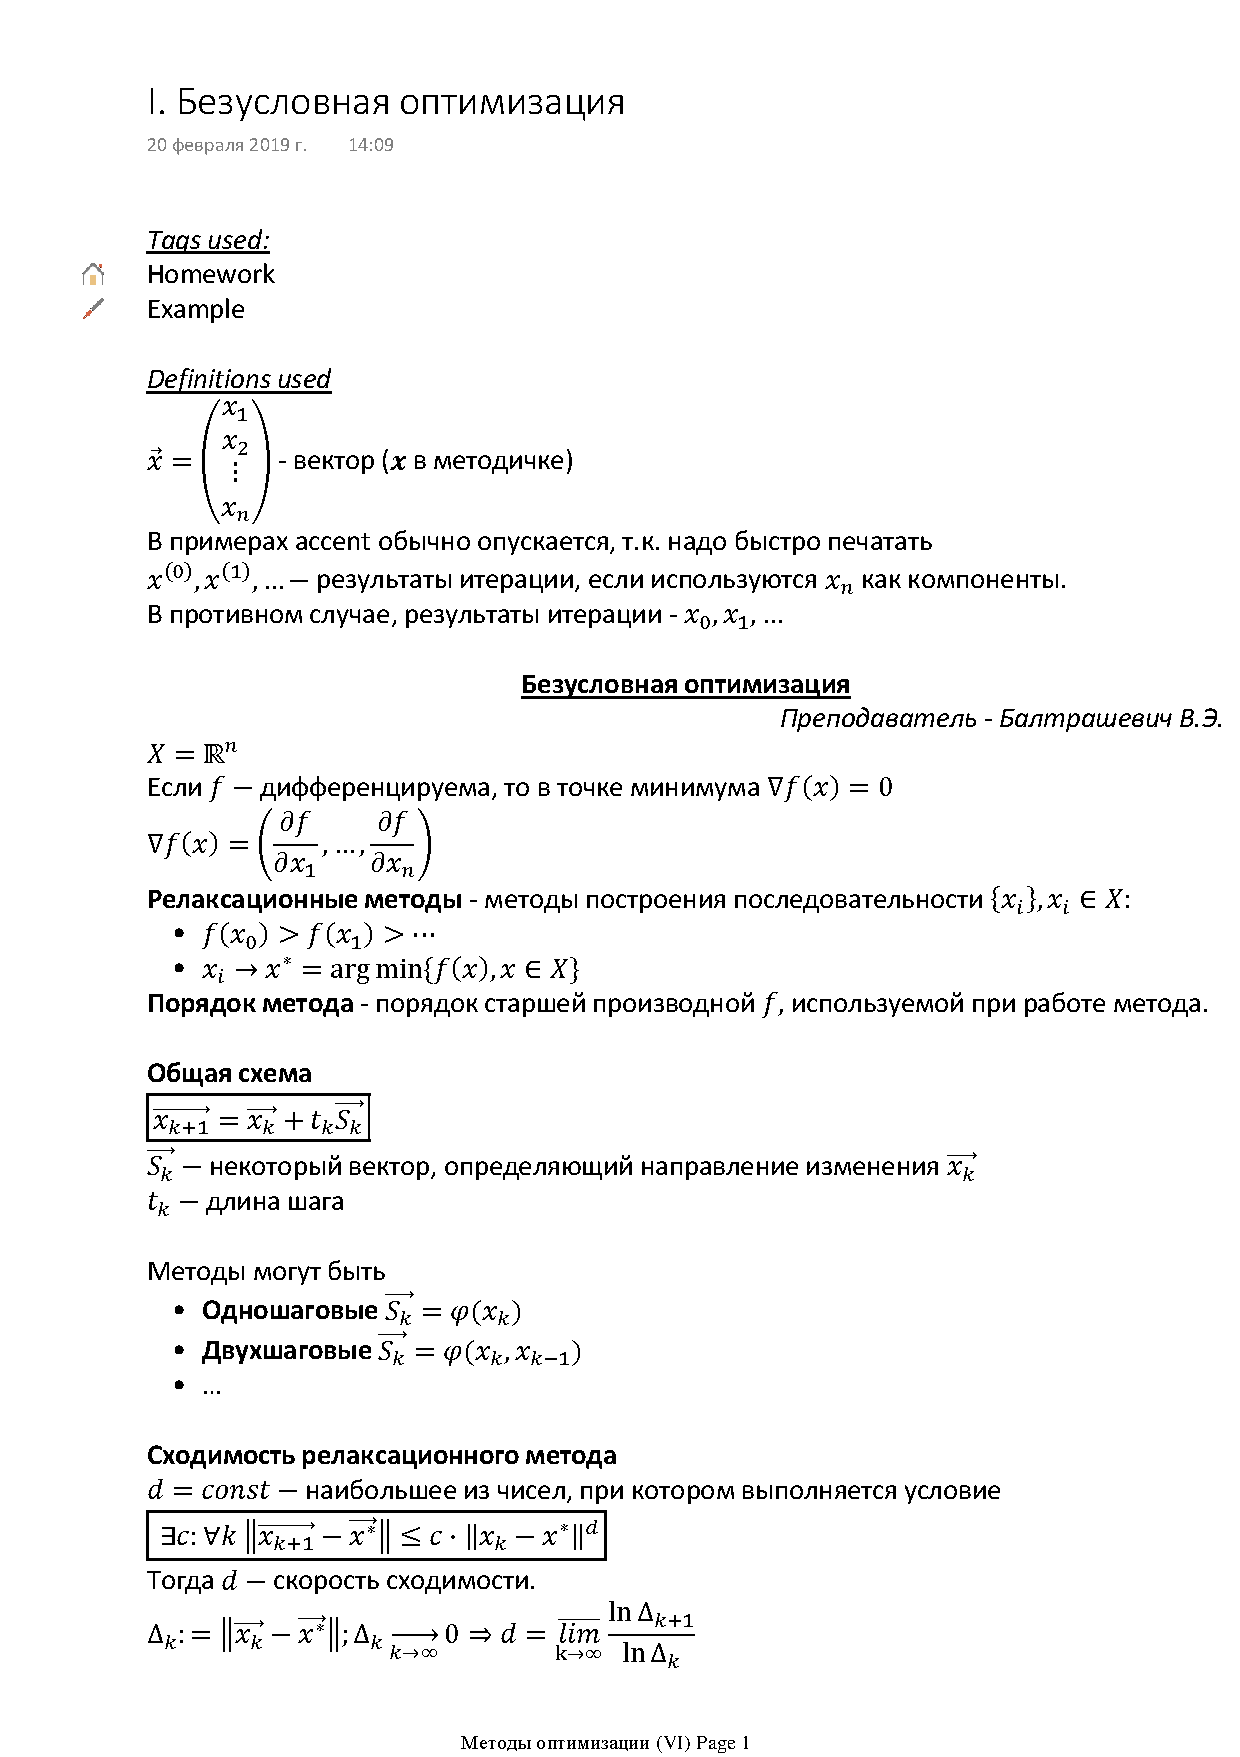
\includepdf[
	pages=-,
	addtotoc={
		1, section, 1, Безусловная оптимизация, l1opt,
		2, subsection, 2, Методы первого порядка, l1grad,
		2, subsubsection, 3, Градиентный метод с постоянным шагом, l1gradconst,
		3, subsubsection, 3, Покоординатный спуск, l1coorddesc,
		3, subsubsection, 3, Выпуклые функции и множества, l1extset,
		6, subsubsection, 3, Метод с дроблением шага; метод наискорейнего спуска, l1quickdesc,
		8, subsubsection, 3, Метод Ньютона, l1newton,
		9, subsubsection, 3, Метод Пауэлла, l1pauell,
		10, subsection, 2, Многошаговые методы, l1multi,
		10, subsubsection, 3, Метод тяжелого шарика, l1ball,
		11, subsubsection, 3, Метод сопряженных градиентов, l1combgrad,
		11, subsubsection, 3, Модификация Полака-Ривьера, l1rivier,
		11, subsection, 2, Квазиньютоновские методы, l1newtonquasi,
		12, subsection, 2, Методы нулевого порядка, l1zeroorder,
        12, subsubsection, 3, Метод симплексов (это не отсюда; но что делать), l1simplex,
		15, subsection, 2, Методы прямого поиска, l1direct		
	}
]{pdf/lec1.pdf}
	
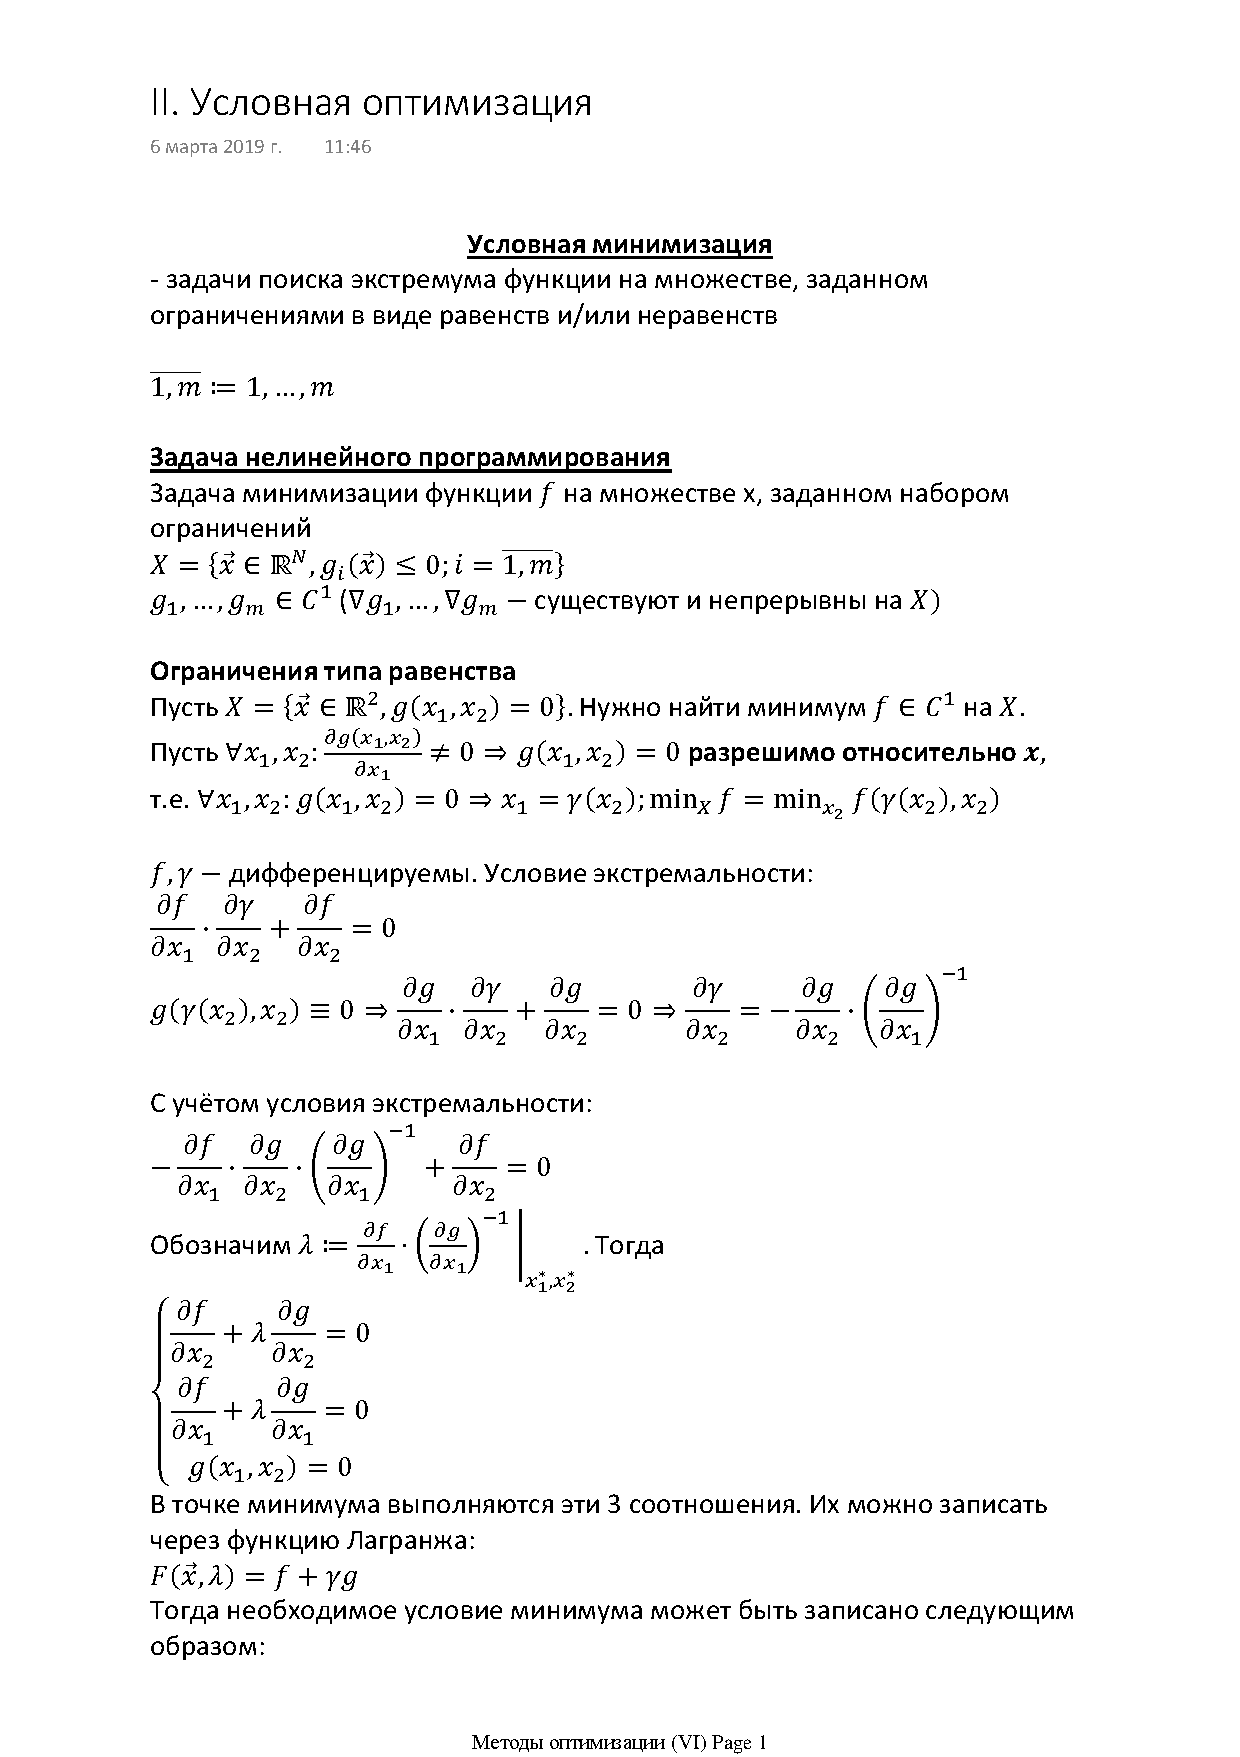
\includepdf[
	pages=-,
	addtotoc={
		1, section, 1, Условная минимизация, l2opt,
		1, subsection, 2, Задача нелинейного программирования, l2nonlinear,
		1, subsubsection, 3, Ограничения типа равенства, l2equlimit,
		2, subsubsection, 3, Ограничения типа неравенств, l2nonequlimit,
		2, subsubsection, 3, Лемма Фаркаша, l2farkash,
		2, subsubsection, 3, Теорема Каруша-Джона, l2farkash,
		4, subsection, 2, Задача выпуклого программирования, l2ext,
		5, subsubsection, 3, Теорема о седловой точке, l2sedl,
		5, subsubsection, 3, Теорема Куна-Таккера, l2kuntakker,
		6, subsection, 2, Методы условной минимизации, l2methods,
		6, subsubsection, 3, Метод проекции градиента, l2gradproj,
		6, subsubsection, 3, Метод условного градиента, l2gradcond,
		7, subsubsection, 3, Метод модифицированной функции Лагранжа, l2lagrange,
		7, subsubsection, 3, Метод штрафных функций, l2fines,
		8, subsection, 2, Двойственность задачи выпуклого программирования, l2double
	}
]{pdf/lec2.pdf}
	
\section{Линейное программирование}
\subsection{Основные понятия}
\textbf{Задача линейного программирования} - поиск минимума линейной функции $f$ на множестве $X=\{ \vec{x} \in \mathbb{R}: g_j (\vec{x}) \le 0, j=1,...,m \}$, где $g_j$ - афинные. ЗЛП - частный случай ЗВП и ЗНП.

Функция - \textbf{линейная}, если
\[
	f(\lambda_1 \vec{x_1} + \lambda_2 \vec{x_2} = \lambda_1 f(\vec{x_1}) + \lambda_2 f(\vec{x_2}); \lambda \in \mathbb{R}, \vec{x_i} \in X
\]
В $n$-мерном пространстве линейная функция может быть определена как:
\[ f(\vec{x}) = (\vec{c}, \vec{x})   \]
\[ f(\vec{x}) = c_1 x_1 + ... + c_n x_n \]
Функция $g$ - \textbf{афинная}, если $g-b$ - линейна для некоторого числа $b$. 
В координатной форме множество $X$ описывается:
\[
	\begin{cases}
		a_{11}x_1 + ... + a_{1n}x_n \le b_1\\
		...\\
		a_{m1}x_1 + ... + a_{mn}x_n \le b_m
	\end{cases}
\]

Если в системе используются только неравенства, \textbf{ЗЛП в стандартной форме}. Если в системе используются только равенства, \textbf{ЗЛП в канонической форме}. 

ЗЛП в канонической форме эквивалентна некоторой задаче в стандартной форме. Чтобы избавится от неравеств, нужно добавить в пространство ещё одну координату
\[
	\begin{cases}
		a_{11}x_1 + ... + a_{1n}x_n + x_{n+1} = b_1\\
		...\\
		a_{m1}x_1 + ... + a_{mn}x_n + x_{n+m} = b_m
	\end{cases}
\]
Ограничения вида $(\lambda, x) = $ можно представить как совокупность $(\vec{\lambda}, \vec{x}) \le 0$ и $(\vec{\lambda}, \vec{x}) \ge 0$. 

Эти же ограничения можно записать в матричном виде: 
\[ X = \{A\vec{x} = \vec{b}, x \ge 0, x \in \mathbb{R} \}  \]
где $A$ - матрица $m \times n$, $x$ - вектор размерности $n$, $b$ - вектор размерности $m$. 

Точка $\vec{x}$ выпуклого множества $X$ называется \textbf{крайней (угловой)}, если 
$
x = \lambda \vec{x_1} + (1 - \vec{x_2}) = \vec{x} \Rightarrow 
\vec{x_1} = \vec{x_2} = \vec{x}.
$, где $\vec{x}, \vec{x_1}, \vec{x_2} \in X, \lambda \in [0, 1]$. 
, т.е. крайнюю точку нельзя выразить с помощью линейной комбинации других точек выпуклого множества.

\paragraph{Теорема} (\textit{О представлении}) Всякая точка допустимого ограниченного
множества ЗЛП допускает представление в виде выпуклой комбинации его
крайних точек. (Без доказательства)

\paragraph{Теорема} (\textit{О существовании оптимальной точки}) Если целевая функция на допустимом множестве ЗЛП ограничена снизу, то оптимальная точка существует. (Без доказательства)

Если допустимое множество $X$ не пусто, то справедлива альтернатива:
\begin{itemize}
	\item $\min\limits_{X} {f(\vec{x})} = -\infty$
	\item $\exists \vec{x}^*: (\vec{c}, \vec{x}^*) = \min\limits_{X} \vec{c}, \vec{x}$ - существует оптимальная точка
\end{itemize}

\subsection{Геометрическая интерпретация ЗЛП}
Пусть $ X = \{A\vec{x} \ge \vec{b}, \vec{x} \ge 0 \}$; $f(\vec{x})=(\vec{c}, \vec{x})$ - целевая функция;
\[
	A = \begin{pmatrix}
		\vec{a_1} \\ \vdots \\ \vec{a_m}
	\end{pmatrix}; \vec{b} = \begin{pmatrix}
		b_1 \\ \vdots \\ b_m
	\end{pmatrix}
\]
где $\vec{a_i}$ - строки длины $n$. В этом случае $i$-е условие принимает вид $(\vec{a}_i, \vec{x}) \ge b_i$. 
Множество точек, для которых справедливо это неравенство - полупространство с граничной гиперплоскостью $(\vec{a}_i, \vec{x}) = b_i$ - пересечение конечного числа полупространств.

\textbf{Гиперплоскость} в $\mathbb{R}^n$ - пространство размерности $\mathbb{R}^{n-1}$
\begin{figure}[h]
	\centering
	\begin{subfigure}[b]{0.45\textwidth}
		\centering
		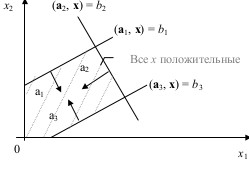
\includegraphics[width=\textwidth]{img/S001.jpg}
		\caption{Ограниченное}
	\end{subfigure}
	\begin{subfigure}[b]{0.45\textwidth}
		\centering
		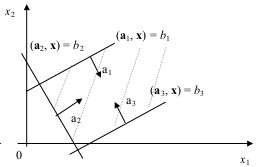
\includegraphics[width=\textwidth]{img/S002.jpg}
		\caption{Неограниченное}
	\end{subfigure}
	\caption{Допустимые множества}
\end{figure}

Введем наряду с множествами целевую функцию:
\begin{figure}[h]
	\centering
	\begin{subfigure}[b]{0.45\textwidth}
		\centering
		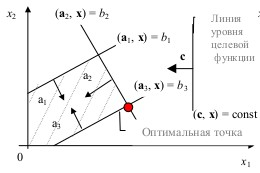
\includegraphics[width=\textwidth]{img/S003.jpg}
		\caption{Есть оптимальная точка}
	\end{subfigure}
	\begin{subfigure}[b]{0.45\textwidth}
		\centering
		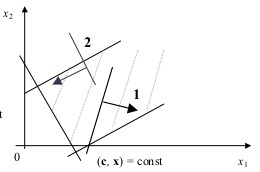
\includegraphics[width=\textwidth]{img/S004.jpg}
		\caption{Минимума нет}
	\end{subfigure}
	\caption{Поиск оптимальной точки}
\end{figure}

\subsection{Условие оптимальности для ЗЛП}
\paragraph{Лемма.} Пусть $\vec{x}^*$ - оптимальная точка ЗЛП, пусть существуют такие точки $\vec{x_1}, ..., \vec{x_m} \in X$, что $ \sum\limits_{i=1}^m \lambda_i \vec{x}_i $, где $\lambda_i > 0$ и $ \sum\limits_{i=1}^m \lambda_i = 1$. Тогда $(\vec{c}, \vec{x}^*) = (\vec{c}, \vec{x_1}) = ... = (\vec{c}, \vec{x_m})$

\subparagraph{Доказательство.} По условию,
$(\vec{c}, \vec{x}^*) \le (\vec{c}, \vec{x}_1), ..., (\vec{c}, \vec{x}^*) \le (\vec{c}, \vec{x_m}).$. По свойству скалярного произведения: 
\[
(\vec{c}, \vec{x^*}) = (\vec{c}, \sum_{i=1}^{m} \lambda_i \vec{x}_i) = \sum_{i=1}^{m} \lambda_i (\vec{c}, \vec{x}) \Rightarrow (\vec{c}, \vec{x}^*) = (\vec{c}, \vec{x_1}) = ... = (\vec{c}, \vec{x_m})
\]

\paragraph{Теорема} (\textit{Об угловой точке}) Если для ЗЛП существует оптимальная точка $\vec{x}^*$, то найдется \textbf{угловая точка} $\vec{x}^0 \in \vec{X}$ такая, что $(\vec{c}, \vec{x}^*) = (\vec{c}, \vec{x}^0)$

\subparagraph{Доказательство}
\begin{enumerate}
	\item Пусть $X$ - ограничено. По теореме о представлении:
	\[
		\vec{x}^* = \sum_{i=1}^n \lambda_i \vec{x_i}; \lambda_i > 0, \sum\limits_{i=1}^n \lambda_i = 1
	\]
	$x_i$ - угловые (крайние) точки множества X.
	В случае необходимости можно перенумеровать $\lambda_i$ так, чтобы $\lambda_1 \ne 0, ..., \lambda_m \ne 0$, $\lambda_{m+1} = 0, ..., \lambda_n = 0$. Тогда 
	Тогда 
	\[
		\vec{x}^* = \sum_{i=1}^m \lambda_i \vec{x_i}; \lambda_i > 0, \sum\limits_{i=1}^m \lambda_i = 1
	\]
	По предыдущей лемме $(\vec{c}, \vec{x}^*) = (\vec{c}, \vec{x_1}) = ... = (\vec{c}, \vec{x_m})$. В качестве крайней можно взять любую угловую точку. 
	\item Пусть $X$ - не ограничено, а $\vec{x}^*$ - оптимальная точка. Выберем некоторое число $ \mu > 0 $ и построим 2 множества:
	\[
		L = \{ \vec{x} \in \mathbb{R}: \sum_{j=1}^{n} \le \mu \}; \ 
		l = \{ \vec{x} \in \mathbb{R}: \sum_{j=1}^{n} = \mu \}
	\]
	\screenshot{width=7cm}{img/S005.jpg}{Вид множеств $L$, $l$}
	
	Число $\mu$ выбирается так, что $\vec{x}^* \in L$, но $\vec{x}^* \notin l$. Тогда $\vec{x}^* \in X \cap L$, которое является ограниченным. Поэтому, по теореме о представлении,
	\[
	\vec{x}^* = \sum_{i=1}^m \lambda_i \vec{x_i}; \lambda_i > 0, \sum\limits_{i=1}^m \lambda_i = 1
	\]
	$\vec{x_i}$ - угловые точки множества $X \cap L$. 
	
	Если хотя бы одна $\vec{x_i} \ne l$, теорема доказана. Иначе, из теоремы оп представлении следует, что $\vec{x}^* \in l$, что противоречит выбору числа $\mu$.
\end{enumerate}

\subsection{Базис и базисное решение}
Пусть $ X = \{\vec{x} \in \mathbb{R}: \sum^{n}_{i=1} a_{ij} x_j = \vec{b_i}, i = 1,m, \ x_j \ge 0 \} $; Требуется найти $ \min\limits_{X} (\vec{c}, \vec{x}) = \min\limits_X \sum^{n}_{j=1} c_j x_j $

Введем векторы: $ \vec{A_j} = (a_{1j}, ..., a_{mj})^T $, $ \vec{B} = (b_1, ..., b_m)^T $, которые называются \textbf{векторами условий}. Тогда ЗЛП имеет вид:
\[ \sum^{n}_{j=1} x_j \vec{A_j} = \vec{B}, x_j \ge 0, j=1,n; \ \min_X (\vec{c}, \vec{x}) = ? \]

Допустимое решение является \textbf{базисным}, если система векторов условий, отвечающих его положительным компонентам, линейно независима. При этом упомянутая система векторов($A_j$) называется \textbf{базисом}.

\paragraph{Теорема} (\textit{О допустимом решении ЗЛП}). Допустимое решение является крайней точкой (\textit{планом}) тогда и только тогда, когда оно базисное.

\subparagraph{Доказательство.} \textit{Достаточность.} Пусть $x$ - базисное решение. Без ограничения общности можно предположить, что первые $k$ компонент $x$ (решения) отличны от нуля, т.е. $\vec{x} = (x_1, ..., x_k, 0, ..., 0)^T$. 

По определению базисного решения $\sum\limits^n_{j=1} x_j \vec{A_j} = \vec{B}$ и система векторов $\vec{A_1},...,\vec{A_k}$ линейно независима. Покажем, что $x$ является крайней точкой. Допустим противное, т.е., что точка $x$ может быть представлена в виде $x = \alpha \vec{x'} + (1-\alpha)\vec{x''}, 0 < \alpha < 1, x', x'' \in X$ - различные точки.

В силу того, что $\alpha > 0, 1 - \alpha > 0$, $x'$ и $x''$ должны иметь вид: 
\[ \vec{x}' = (x_1', ..., x_k', 0, ..., 0)^T; \ \vec{x}''=(x''_1, ..., x''_k, 0, ..., 0)^T \]

Так как $ \vec{x}' $, $\vec{x}''$ - допустимые точки, то $\sum\limits^n_{j=1} x'_j \vec{A_j} = \vec{B}$, $\sum\limits^{n}_{j=1} x''_j \cdot \vec{A_j} = \vec{B}$, следовательно $\sum\limits^n_{j=1} (x'_j - x''-j) \vec{A_j} = 0$

Из линейной независимости $\vec{A_1}, ..., \vec{A_k}$ следует, что $\vec{x}' = \vec{x}''$ - крайняя точка.

\textit{Необходимость}. Пусть $\vec{x} = (x_1, ..., x_k, 0, ..., 0)^T $ является крайнейточкой $X$. Покажем, что $x$ является базисным решением. Для этого достаточно показать, что система векторов $\vec{A_1}, ..., \vec{A_k}$ линейно независима.

Предположим противное. Тогда $\exists \alpha_j \ne 0$, такие, что $\sum\limits_{j=1}^k \alpha_j \vec{A_j} = 0$. Так как $\vec{x}$ - допустимое решение, то $ \sum\limits^{k}_{j=1} x_j \vec{A_j} = \vec{B} $. 

Рассмотрим при произвольном $\varepsilon > 0$ следующие выражения: 
\[ \sum^{k}_{j=1} (x_j + \varepsilon \alpha_j) \vec{A_j} = \vec{B} \
\sum^{k}_{j=1} (x_j - \varepsilon \alpha_j) \vec{A_j} = \vec{B} \]

Ясно, что $\varepsilon$ можно подобрать так, чтобы точки 
\[ \vec{x}' = (x_1 + \varepsilon \alpha_1, ..., x_k + \varepsilon \alpha_k, 0, 0)^T, \ 
x''=(x_1 = \varepsilon \alpha_1, ..., x_k - \varepsilon \alpha_k, 0, 0)^T\]
имели положительные компоненты, т.е. были бы допустимыми решениями. В таком случае
$ \vec{x} = \frac{\vec{x}'+\vec{x}''}{2}$, т.е. $x$ - не крайняя точка. В таком случае предположение неверно, и $ \vec{A_1}, ..., \vec{A_k} $ линейно независимы.

\paragraph{Следствие 1.} Так как векторы $ \vec{A_1}, ..., \vec{A_n}$ имеют размерность $m$, то крайняя точка, принадлежащая $X$, имеет не более чем $m$ положительных компонент.

\paragraph{Следствие 2.} Каждой угловой точке соответствует не более $m$ ($k \le m$) линейно независимых векторов системы $A_1, ..., A_n$. 

\paragraph{Следствие 3.} Число крайних точек множества $X$ конечно.

\subsection{Симплекс-метод решения ЗЛП}
Задача линейного программирования:
\begin{equation}
    \label{eq:simplex:task}
    X = \{ \vec{x} \in \mathbb{R} : A \vec{x} \ge \vec{b}, x \ge 0 \}
\end{equation}

Симплекс метод решения ЗЛП состоит из двух этапов:
\begin{enumerate}
    \item Поиск крайней точки допустимого множества
    \item Перебор крайних точек с целью поиска оптимальной
\end{enumerate}


\textbf{1. Поиск крайней точки допустимого множества.}\\
Расширим пространство состояний. Введем дополнительные координаты
\begin{equation}
    \label{eq:simplex:task2}
X = \{ \vec{x} \in \mathbb{R}^n: A \vec{x} - \vec{y} = \vec{b}, x \ge 0, y \ge 0 \}, \ \min_X ( \vec{c}, \vec{x}) = ? 
\end{equation}

Задачи \ref{eq:simplex:task}, \ref{eq:simplex:task2} эквивалентны, т.к. двойственной к обеим задачам будет $ max( \vec{b}, \vec{\lambda} ) $ при $ A^T \vec{\lambda} \le c, \lambda \ge 0 $
\begin{align*}
    1y_1 + 0 + ... + 0 &= a_{11}x_1 + ... + a_{1n}x_n-b_1 \\
    0 + 1y_2 + ... + 0 &= a_{21}x_1 + ... + a_{2n}x_n-b_2 \\
    ... &... ...\\
    0 + 0 + ... + 1y_m &= a_{m1}x_1 + ... + a_{mn}x_n-b_m
\end{align*}

Переменные $y_1,...,y_n$ можно рассматривать как базисные переменные, т.к. соответсвующие им векторы условий линейно независимы ($ \vec{Y_1},..., \vec{Y_m} $).

Есть $n+m$ переменных и $m$ уравнений. Тогда $x_1,...,x_n$ можно рассматривать как свободные переменные, которые могут принимать произвольные значения. Как было показано ранее, для того, чтобы точка увеличенного пространства $ (\vec{x}, \vec{y})^T $ была крайней, достаточно положить $\vec{x}=0$, поэтому полагаем $ x_1 := ... x_n := 0 $. 

Если все $y_i = -b_i \ge 0$, получим крайнюю точку допустимого множества. Если хотя бы один $y_i$ отрицателен, меняем систему координат.

\subparagraph{Переход к новому базису. } Обозначим полученную крайнюю точку
$\vec{x}' = (y_1 = -b_1, ..., y_m=-b_m, x_1=0,...,x_n=0)$. Ей соответствует разложение по базису:
\begin{equation}
    \label{eq:simplex:basis}
    y_1 + \vec{Y_1} + y_2 \vec{Y_2} + ... + y_m \vec{Y_m} = \vec{B}
\end{equation}
Разложим по базису каждый $\vec{A_j}, \ j= \overline{1,n}: \sum\limits^{m}_{i=1} a_ij \vec{Y_i} $,

Предположим, что для некоторого вектора, не входящего в базис (например, $\vec{A_s}$) положителен хотя бы один из коэффициентов $a_is$ в разложении
\begin{equation}
    \label{eq:simplex:basis2}
    a_1s + \vec{Y_1} + a_{2s} \vec{Y_2} + ... + a{ms} \vec{Y_m} = \vec{A_s}
\end{equation}

Зададимся значением $\Theta > 0$. Умножим на него обе части равенства \ref{eq:simplex:basis2} и вычтем результат почленно из равенства \ref{eq:simplex:basis}. Получим:
\begin{equation}
    \label{eq:simplex:res1}
    (y_1 - \Theta a_{1s}) \vec{Y_1} + (y_2 - \Theta a_{2s}) \vec{Y_2} + ... + 
    (y_m - \Theta a_{ms}) \vec{Y_m} + \Theta \vec{A_s} = \vec{B}
\end{equation}
Получается, что вектор $ \vec{x}'' = (y_1 - \Theta a_{1s}, ..., y_m - \Theta a_{ms}, 0, ..., 0, \Theta_s, 0, ...,0) $ является допустимой крайней точкой, если его компоненты неотрицательны. Так как $\Theta >0$, то все компоненты вектора $ \vec{x}' $, в которые входят $a_{is} < 0$, положительны. Поэтому надо рассмотреть только компоненты, включающие положительные $a_{is}$. Т.е. надо определить такое $\Theta>0$, при котором для всех $a_is>0$ будет
\[y_i - \Theta a_{is} \ge 0 \Rightarrow 0 \le \Theta \le \frac{y_i}{a_is}
\Rightarrow \Theta \le \min_{i: a_{is} > 0} \frac{y_i}{a_{is}}\]
Поскольку крайняя точка не может содержать $m+1$ положительную компоненту, в $\vec{x}''$ нужно обнулить по крайней мере одну положительную компоненту. Поэтому надо положить:
\[ \Theta = \Theta_0 = \min_{i: a_is > 0} \frac{y_i}{a_{is}} = \frac{y_i}{a_{rs}}  \]
И $r$-я компонента обратится в 0. Полученное значение подставим в \ref{eq:simplex:res1}:
\[ (y - \frac{y_r}{a_{rs}} a_{1s} \vec{Y_1}) + ... + (y_r - \frac{y_r}{a_{rs}} a_{rs}) + ... + (y_m - \frac{y_r}{a_{rs}} a_{ms} \vec{Y_m}) + ... + \frac{y_r}{a_{rs}} \vec{A_s} = \vec{B} \]

В результате получается новое разложение:
\[ y'_1 \vec{Y_1} + ... + 0 \vec{Y_r} + ... + y\_m \vec{Y_m} + y'_s \vec{A_s} = \vec{B} \]
которому соответствует новая крайняя точка $\vec{x}'' = (y'_1, ..., 0, ...,y'_m, 0, ..., 0, y'_s, 0, ..., 0) $, где $y'_i=y_i - \Theta_0 a_{is}, i=\overline{1,m}, i \ne r, y'_s = \Theta_0$.

Рассмотрен переход от одной крайней точки к другой. Если на первом этапе симплекс-метода получается, что $-b_i < 0$, то нужно пользоваться формулой:
\[ \Theta_0 = \max_{i: \frac{-b_i}{a_{is}} < 0} \frac{-b_i}{a_{is}}  \]

Нужно осуществить преобразовие для всех векторов. Если при поиску допустимой крайней точке хотя бы один из $y_i<0$, то необходимо изменить систему координат, т.е. перейти в другую крайнюю точку. 

Пусть с помощью предыдущих рассуждений выбрали столбец $s$ и строку $r$, т.е. будем ввводит в базис $x_s$ и выводить из базиса $y_r$.
\[ y_r=a_{r1} x_1 + ... + a_{rs}x_s + ... + a_{rn} x_n - b_r \]
Так как в базис вводится $x_s$, коэффициент при нём должен быть 1, а во всех остальных уравнения он должен быть 0. Вычислим $x_s$:
\begin{equation}
    \label{eq:simplex:xs}
    x_s = \frac{b_r}{a_{rs}}  - \sum^{n}_{j=1; j\ne s} \frac{a_{rj} x_j}{a_{rs}} + \frac{y_r}{a_{rs}}  
\end{equation}
Подставив эту координаты во все остальные ограничения, получается:
\begin{equation}
    \label{eq:simplex:yi}
    y_i = \sum^n_{j=i, j \ne s} \left( a_{ij} - \frac{a_{is} a_{rj}}{a_{rs}} \right) x_s + \frac{a_{is}}{a_{rs}} y_r - b_i  + \frac{a_{is}}{a_{rs}} b_r 
\end{equation}

Табличный метод - см. \ref{l1simplex}.

\subsection{Транспортная задача}
Некоторый однородный продукт сосредоточнен у $m$ поставщиков в количестве $a_i$ ($i= \overline{1,m} $) единиц. Необходимо доставить $n$ потребителям $B_j$ в количестве $b_j$ ($j = \overline{1,n} $) единиц этого продукта. Известно, что $c_{ij}$ - стоимость перевозки единицы груза от $i$-го поставщика к $j$-му потребителю. Необходимо составить план перевозок, позволяющий вывести все грузы, полностью удовлетворить потребности, имеющий минимальную стоимость.

Пусть $x_{ij}$ - количество единиц груза, запланированного к перевозке от $i$-го поставщика к $j$-му потребителю.

Надо найти минимум $\min \sum\limits^{m}_{i=1} \sum\limits^{n}_{j=1} c_{ij}x_{ij} $, причем:
\begin{itemize}
    \item $ \sum\limits^{n}_{j=1} x_{ij} = a_i, \ i=\overline{1,m} $ - все грузы должны быть вывезены,
    \item $ \sum\limits^{m}_{i=1} x_{ij} = b_j, \ j= \overline{1,n}  $ - все потребители должны быть удовлетворены
    \item $x_{ij} \ge 0, i = \overline{1,m}, j= \overline{1,n}  $
\end{itemize}

Если $ \sum\limits^{m}_{i=1} a_i = \sum\limits^{n}_{j=1} b_j $, то модель называется \textbf{закрытой}. Можно показать, что любая закрытая транспортная задача имеет решение.

Транспортная задача - ЗЛП, но специфичная формой ограничений. Матрица ограничений имеет n+m строк:

1-я группа ограничений:
\begin{equation}
\label{eq:transp:limg1}
\begin{matrix}
        x_{11} + x_{12} + ... + x_{1n} & & & =a_1 \\
    & x_{21} + x_{22} + ... + x_{2n} & & = a_2 \\
    \hdotsfor{4}\\
    & & x_{m1} + x_{m2} + ... + x_{mn} & =a_m
\end{matrix}
\end{equation}
2-я группа ограничений:
\begin{equation}
\label{eq:transp:limg2}
\begin{matrix}
        x_{11} + & & & x_{21} + & & & x_{m1} & & & =b_1\\
      & x_{12} + & & & x_{22} + & & & x_{m2} & & =b_2\\
      \hdotsfor{10}\\
    & & x_{1n} + & & & x_{2n} + & & & x_{mn} & =b_n
\end{matrix}
\end{equation}
Нетрудно заметить, что матрица сильно разрешена. Например, для $n=2, m=3$:
\[ A = \begin{pmatrix}
    1 & 1 & 0 & 0 & 0 & 0\\
    0 & 0 & 1 & 1 & 0 & 0\\
    0 & 0 & 0 & 0 & 1 & 1\\
    1 & 0 & 1 & 0 & 1 & 0\\
    0 & 1 & 0 & 1 & 0 & 1
\end{pmatrix}; \ b = \begin{pmatrix}
    a_1 \\ a_2 \\ a_3 \\ b_1 \\ b_2
\end{pmatrix} \]
Поэтому симплекс-метод будет работать очень медленно.

\subsubsection{Построение первоначального опорного плана}
В транспорной задаче $ m \times n$ неизвестных и $m+n$ уравнений. Если сложить почленно системы \ref{eq:transp:limg1} и \ref{eq:transp:limg2}, то получится 2 одинаковых уравнения, т.е. система линейно зависима. 

Отбросим одно из уравнений системы. В общем случае система ограничений должна содержать $m+n-1$ линейно независимых уравнений, следовательно, невырожденный опорный план транспортной задачи содержит $m+n-1$ положительных компонент или перевозок (остальные равны 0). Рассмотрим конкретный пример
\screenshot{width=\textwidth}{img/S006.jpg}{Матрица планирования}
В таблице должно быть $m+n-1$ (здесь - $6$) занятых клеток ($>0$). Занятые клетки соотвествуют базисным неизвестным. Опорность (допустимость) плана заключается в ацикличности, т.е. в таблице нельзя построить замкнутый цикл, все вершины которого лежат в занятых клетках.

\textbf{Цикл} - набор клеток вида $(i_1, j_1), (i_1, j_2), (i_2, j_2), ..., (i_m, j_1)$, в котором каждые последующие 2 клетки располагаятся в одном столбце, причем последняя клетка находится в той же строке или столбце, что и первая. Если цикл не найдет, план является опорным. 

\paragraph{Метод минимальной стоимости.} Один из методов построения первоначального плана. Из таблицы выбивается наименьшая стоимость, и в нужную клетку поменьшается $\min (a_i, b_j)$. Из рассмотрения исключается строки и столбцы с $a_i = 0$ и $b_j=0$. 
Процесс продолжается, пока все запасы не будут распределены, а потребности - удовлетворены. 

Для примера матрица стоимостей и результата метода:
\[
\begin{array}{c|cccc|c}
    & B_1 & B_2 & B_3 & B_4 & a \\
    \hline
    A_1 & 5 & 1 & 4 & 7 & 5\\
    A_2 & 2 & 6 & 10 & 3 & 7\\
    A_3 & 4 & 2 & 3 & 2 & 4\\
    \hline
    b & 3 & 8 & 2 & 3 & 
\end{array}; \ \ 
\begin{array}{c|cccc|c}
& B_1 & B_2 & B_3 & B_4 & a \\
\hline
A_1 & & 5 & & & 5\\
A_2 & 3 & & 2 & 2 & 7\\
A_3 & & 3 & & 1 & 4\\
\hline
b & 3 & 8 & 2 & 3\\
\end{array} \]
\[ 1 \cdot 5 + 3 \cdot 2 + 2 \cdot 10 + 2 \cdot 3 + 3 \cdot 2 + 1 \cdot 2 = 45 \]

\subsubsection{Метод потенциалов}
\paragraph{Лемма.} Если при подстановке компонент оптимального плана в систему ограничений исходной задачи $i$-е ограничение обращается в неравенство, то $i$-я компонента оптимального плана двойственной задачи равна $0$. \\
Если $i$-я компонента оптимального плана двойственной задачи положительна, то $i$-е ограничение исходной задачи удовлетворяется её оптимальным решением, как строгое равенство. 

\paragraph{Теорема.} Если план $x^*$ является оптимальным, ему соответствует система из $m+n$ чисел $u_i$ и $v_j$, удовлетворяющая условиям:
\[ \begin{cases}
        u_i + v_j = c_{ij}, \ \textrm{для} \ x_{ij}^* > 0\\
        u_i + v_j \le c_{ij}, \ \textrm{для} \ x_{ij}^* = 0
\end{cases}\]

\subparagraph{Доказательство.} Вместо решения исходной транспортной задачи решаем двойственную.
ЗЛП: $\min ( \vec{c}, \vec{x}) -?; \ A \vec{x} = \vec{E}, \ \vec{x} \ge 0; \vec{E} = (a_1, ..., a_m, b_1, ..., b_n)^T $

Двойственная: $\min ( \vec{E}, \vec{\lambda}) - ? ; \ A^T \lambda \le \vec{c}, \lambda \ge 0$ 
Так как в строке $A^T$ два ненулевых элемента $u_i = \lambda_i, v_j = \lambda_j$, получаем $u_i + v_j \le c_{ij} $.

С учетном леммы двойственную задача можно записать в виде:
\[ \max \left( \sum^m_(i=1) a_i u_i + \sum^{n}_{j=1} b_j v_j \right)\] 
    где $\ u_j + v_j = c_{ij}$ для  $x^*_{ij} > 0$, $u_i + v_j \le c_{ij}$ для $x^*_{ij} = 0 $.
Теорема доказана.

Таким образом, для того, чтобы план был оптимальным, необходимо выполнение следующих условий:
\begin{itemize}
    \item Для любой занятой клетки $u_i + v_j = c_{ij}$
    \item Для любой незанятой $u_i+v_j \le c_{ij}$
\end{itemize}
Если хотя бы для одной клетки не удовлетворяется условие $u_i + v_j \le c_{ij}$, то план не является оптимальным и его можно улучшить, введя в базис вектор, соответствующий клетке, для которой нарушается условие оптимальности.

\paragraph{Алгоритм метода потенциалов. } 
\begin{enumerate}
    \item Построение системы потенциалов из условия $u_i + v_j = c_{ij}$ для занятых клеток. Поскольку уравнений не хватает, обнулить любую компоненту. Сделав $u_2=0$, получим
    \[ \begin{cases}
        u_1 + v_2 = 1\\
        u_2 + v_1 = 2\\
        u_2 + v_3 = 10\\
        u_2 + v_4 = 3\\
        u_3 + v_2 = 2\\
        u_3 + v_4 = 2\\
    \end{cases}; \ \
    \begin{array}{ccccc|cc}
        & & & & & u & \\
        & & & & & -2 & (1)\\
        & & & & & 0 & (2)\\
        & & & & & -1 & (3)\\
        \hline
        v & 2 & 3 & 10 & 3 & &\\
          & (1) & (2) & (3) & (4)
    \end{array} \]
    \item Проверка условия оптимальности для незанятых клеток\\
    Характеристические разности: $q_{ij} = u_i + v_j - c_{ij}$. Если в любой незанятой клетке $q_{ij} \le 0$, то конец.
    \[ Q = \begin{array}{c|cccc|c}
            & B_1 & B_2 & B_3 & B_4 & b\\
        \hline
        A_1 & -5 & & +4 & -4 & 5 \\
        A_2 & & -3 & & & 7\\
        A_3 & -3 & +6 & & 4\\
        \hline
        b & 3 & 8 & 2 & 3
    \end{array} \]
\item Выбор клетки, в которую необходимо послать перевозку. Для этого среди $q_{ij} \ge 0$ выбрать максимальную
    \item Построение цикла и определение величины перераспределения груза.\\
    Найденная клетка отмечается плюсом. Теперь занятых клеток $m+n$, т.е. существуюет цикл. Нужно пройти по циклу, чередуя плюсы и минусы.
    \[ \begin{array}{c|cccc|c}
            & B_1 & B_2 & B_3 & B_4 & b\\
        \hline
        A_1 & & & & & 5 \\
        A_2 & & & - & + & 7\\
        A_3 & & & + & - & 4\\
        \hline
        b & 3 & 8 & 2 & 3
    \end{array} \]
    По минусам, найденным ранее, значение $\Theta_0 = \min\limits_{(-)} x_{ij}$ записвается в незанятую клетку. Затем, идя по циклу, сделать $x_{ij} + \Theta_0$ там, где $+$ и $x_{ij} - \Theta_0$ там, где $i$.
    Для рассматриваемого примера $\Theta_0 = 1$ и новые значения:
    \[ \begin{array}{c|cccc|c}
            & B_1 & B_2 & B_3 & B_4 & b\\
        \hline
        A_1 & & 5 & & & 5 \\
        A_2 & 3 & &  1 & 3 & 7\\
        A_3 & & 3 & 1 & & 4\\
        \hline
        b & 3 & 8 & 2 & 3
    \end{array} \]
    \[ f = 5 \cdot 1 + 3 \cdot 2 + 1 \cdot 10 + 3 \cdot 3 + 3 \cdot 2 + 1 \cdot 3 = 39 \]
    Значение функции уменьшилось.
    \item Новый план проверяется на оптимальность, и, в случае необходимости, переход к п. 1.
\end{enumerate}
\section{Вариационное исчисление}
    Задача вариационного исчисления - поиск экстремумов функционалов, аргументами которых являются функции. Требуется найти минимум
    \[ J(y(x)) = \int_a^b f(x,y(x),y'(x))dx \]
    по множеству дважды дифференцируемых функции $y$ с краевыми условия $y(a)=y_0, y(b)=y_1$.
    Определение нормы на множестве: $\lVert y(x) \rVert = \max\limits_{a < x < b}$ \{ |y(x)| + |y'(x)| \}. 

    Пусть $y^*(x)$ доставляет минимум $J(y(x))$.

    Рассмотрим $y(x)=y^*(x)+\varepsilon(x)$, где $\varepsilon(a) = \varepsilon(b)=0$, и $\varepsilon$ - гладкая функция, которая называется \textbf{вариацией}. 

   Пусть $y_\alpha = y^* + \alpha \varepsilon$, тогда
   \[ J(y_\alpha(x)) = \int_a^b f(x, y^* + \alpha \cdot \varepsilon, y'^* + \alpha \cdot \varepsilon' ) dx \ge J(y^*(x)), \]
    так как $y^*$ - аргумент минимума функционала. Из этого неравенства можно получить необходимые условия экстремума.

    \subsection{Уравнение Эйлера-Лагранжа}
    \paragraph{Лемма Дюбуа-Раймона.} Пусть для некоторой функции $f$, непрерывной на $[a,b]$, и для всех функций $h$, непрерывных на $[a,b]$ вместе со своими производными и таких, что $h(a)=h(b)=0$, справедливо: 
    \[ \int_a^b f(x)h(x) = 0 \Rightarrow f \equiv 0 \]
    Разложим $J(y_\alpha(x))$ в ряд Тейлора в окрестности точки $\alpha = 0$:
    \[ J(y_\alpha(x)) = J(y^*) + \alpha \frac{\partial J}{\partial \alpha} + o(\alpha) \]
    $\delta \dfrac{\partial J}{\partial \alpha}$ - первая вариация функционала 
    При фиксированных $y^*(x)$ и $\varepsilon(x)$ функционал зависит от параметра $\alpha$ и необходимым условием экстремума функционала является.
    \[ \left. \frac{\partial J}{\partial \alpha} \right|_{\alpha = 0} = 0 \Rightarrow \delta J = 0 \]
    Получим необходимое условие экстремума функционала в более конструктивной форме. Функционал $J$, рассматриваемый как функция от $\alpha$, может быть записан в виде:
    \[ J(\alpha) = \int_a^b f(x, y(x) + \alpha \varepsilon(x), y'(x) + \alpha \varepsilon'(x)) dx \]
    Тогда необходимое условие экстремума:
    \[ \left. \frac{\partial J (\alpha)}{\partial \alpha} \right|_{\alpha = 0}
        = \int^b_a \left[ \frac{\partial f(x, y, y'}{\partial y} \varepsilon(x) + \frac{\partial f(x,y,y')}{\partial y'} \varepsilon'(x) \right] dx = 0 \]
    \[ \int^b_a \frac{\partial f}{\partial y'} \varepsilon'(x) dx = 
        \underbrace{\left. \frac{\partial f}{\partial y'} \varepsilon(x) \right|_a^b}_{=0} - 
    \int^b_a \varepsilon(x) \frac{d}{dx} \frac{\partial f}{\partial y'} dx \]
    $=0$, т.к. $\varepsilon(a)=\varepsilon(b)=0$
    \[ \frac{\partial J(\alpha)}{\partial \alpha} = 
    \int_a^b \left( \frac{ \partial f(x,y,y') }{\partial y} - \frac{d}{dx} \cdot \frac{\partial f(x, y, y')}{\partial y'} \right) \varepsilon(x)dx=0\]
    Это справедливо с учётом $\varepsilon(a)=\varepsilon(b)=0$. Отсюда с учётом леммы следует:
    \[ \frac{\partial f(x,y^*,y'^*)}{\partial y} - \frac{d}{dx} \frac{\partial f(x, y^* y'^*)}{\partial y'} \equiv 0 \]
    - \textbf{уравнение Эйлера-Лагранжа}
    
    Всякое решение уравнения Эйлера-Лагранжа называется \textbf{Экстремалью}. Функция, доставляющая экстремум функционалу, находится среди экстремалей. Уравнение Эйлера-Лагранжа - необходимое условие экстремума. 

    Одно из достаточных условий локального минимума - \textbf{условие Лежандра}:
    \[ \frac{\partial^2 f(x, y^*(x), y'^*(x))}{\partial y' \partial y'} > 0  \]
    Обозначим $f_y= \frac{\partial f}{\partial y}$, $f_x = \frac{\partial f }{\partial x} $. Тогда уравнение Эйлера-Лагранжа:
    \[ f_y - \frac{d}{dx} f_{y'} = 0 \]

    Раскроем второй член по формуле дифференцирования сложной функции:
    \[ \frac{d}{dx} f_{y'} = \frac{\partial f_{y'}}{\partial x} \cdot \frac{dx}{dx} + \frac{\partial f_{y'}}{\partial y} \cdot \frac{dy}{dx} + \frac{\partial f_{y'}}{\partial y'} \cdot \frac{dy'}{dx} \]
    Тогда уравнение:
    \[ f_y - f_{y'x} - f_{y'y} \cdot y' - f_{y'y'}y'' = 0 \]
    Это нелинейное дифференциальное уравнение второго порядка, поэтому его решение затруднено.
    \subsubsection{Частные случаи уравнения Эйлера-Лагранжа}
    \begin{enumerate}
        \item $f(x,y)$
            \[ \frac{\partial f(x,y)}{ \partial y' } = 0 \Rightarrow \frac{ \partial f(x,y) }{ \partial y} \equiv 0  \]
        \item f(x, y')
        \[ \frac{f}{y} = 0 \Rightarrow \frac{d}{dx} \cdot \frac{ \partial f}{ \partial y' } \equiv 0 \Rightarrow \frac{ \partial f }{ \partial y' } = const \]
        \item $f(y, y')$
        \[ f_y - f_{y'y}y' - f_{y'y'}y'' \equiv 0 \]
        \[ \frac{d}{dx} (f - f_{y'}y') \equiv 0 \Rightarrow f - f_{y'}y' = const \]
    \end{enumerate}
    
    \subsubsection{Задача о брахистохроне}
    Как выбрать профиль горки, чтобы шарик скатился с нёё за минимальное время? Трение отсутствует,  $v$ - скорость, $\varphi$ - угол наклона горки, $g$ - ускорение свободного падения.
    \begin{equation}
        \label{eq:brahv1}
        dx = v \cos \varphi dt 
    \end{equation}
    \begin{equation}
        \label{eq:brahv2}
        \tan \varphi = y'(x) \Rightarrow \frac{1}{\sqrt{1 + (y'(x)^2)}}  
    \end{equation}
    Из закона сохранения энергии:
    \begin{equation}
        \label{eq:brahenergy}
        \frac{mv^2}{2} = mgy \Rightarrow v = \sqrt{2gy} 
    \end{equation}
    Подстави \ref{eq:brahv2}, \ref{eq:brahenergy} в \ref{eq:brahv1}, получим
    \[ \frac{dx}{\sqrt{2gy}} \sqrt{1+y'^2} \]
    Проинтегрируем обе части:
    \[ \int_0^{x_k} \underbrace{ \frac{\sqrt{1+y'^2}}{\sqrt{2gy}}}_F dx = T \]
    Здесь $T$ - время спуска шарика. $F$ зависит от $y$ и $y'$, т.е. это третий частный случай уравнения Эйлера-Лагранжа - $F-y'F_{y'} \equiv const$. $2g$ можно вынести из рассмотрения, т.к. оно не влияет на экстремум.

    \[ \frac{\sqrt{1+y'^2}}{\sqrt{y}} - y' \frac{1}{2} \cdot \frac{2y'}{\sqrt{1+y'^2}} \cdot \frac{1}{\sqrt{y}} \equiv const \]
    
    Приведем к общему знаменателю:
    \[ \frac{1}{\sqrt{y(1+y'^2)}} \equiv const \]
    Пусть $c = \frac{1}{const^2} \Rightarrow const = \frac{1}{\sqrt{c}} $. Тогда 
    \[ y(1+y'^2) \equiv c \]
    Делаем подстановку: \[ y' = \tan{t} \Rightarrow 1 + y'^2 = \frac{1}{\cos^2 t}  \]
    Получается $y=c \cos^2{t}$. Найдем выражение для $x$:
    \[ \begin{rcases*}
        dy = \tan{t} td \\
        B
        C
        dy = 2c \cos t(-\sin{t})dt
\end{rcases*} \Rightarrow dx = 2c(-\cos^2 t) dt \]
    
    Интегрируем:
    \[ x = -2c \int \cos^2 t dt = -2c \int \frac{1-\cos 2t}{2} dt = -ct-c/2 \sin 2t \]
    Полученная кривая - \textbf{циклоида}. 
    \screenshot{width=6cm}{img/S007.jpg}{Результат решения}
	
    \subsection{Вариационные задачи на условные экстремум}
    Будем считать, что $y$ - вектор-функция из $m$ компонент: $y=(y_1, ..., y_m)^T$. Если они независимы, то уравнение Эйлера-Лагранжа надо писать для каждой компоненты $y_i$ отдельно. Если между $y_i$ есть связь, то получаем задачу на условный экстремум.

    \subsubsection{Модельные задачи на условный экстремум}
    \begin{enumerate}
        \item \textbf{Геодезическая линия.} Пусть поверхность задана уравнением $\phi(y_1,y_2,x)=0$, где $\phi$ - дифференцируемая функция, $x$ - независимая координата, $y_1, y_2$ - функции от $x$. Тогда длина пути, соединяющего 2 точки:
        \[ \int_{x_0}^{x_k} \sqrt{1 + y'^2_1 + y'^2_2} dx \]
        Условия здесь - начало и конец геодезической линии
        \item \textbf{Изопериметрическая задача.} Требуется найти линию заданной длины, ограничивающую максимальную площадь. Задача может быть поставлена так: на множестве дифференцируемых функций $y$ с заданными граничными точками, удовляющих равенству, 
        \[ \int_{t_0}^{t_k} \sqrt{y'^2(t) + x'^2(t)} dt = l \]
        Нужно найти максимум фунционала:
        \[ S = \int_{t_0}^{t_k} y(t)x'(t)dt \]
    \end{enumerate}
    Связи типа 1 - \textbf{локальные}, 2 - \textbf{интегральные}. Эти задачи решаются методом множителей Лагранжа.

    \subsubsection{Метод множителей Лагранжа}
    Локальные ограничения: $\varphi_i(x,y,y')=0, i=\overline{1,k} $ - сильные связи\\
    Интегральные: $\int \psi (x,y,y')dx =l, l=\overline{1,p}$ - слабые связи.
    Составим функционал $F^*$:
    \[ F^* = F + \sum^k_{i=1} \lambda_i(x)\varphi(x, y, y') + \sum^p_{j=1} \lambda_{k+j} \psi_j (x, y, y') \]
    
    Количество неизвестных функций увеличилось за счёт введения множителей $\lambda_i$. 

	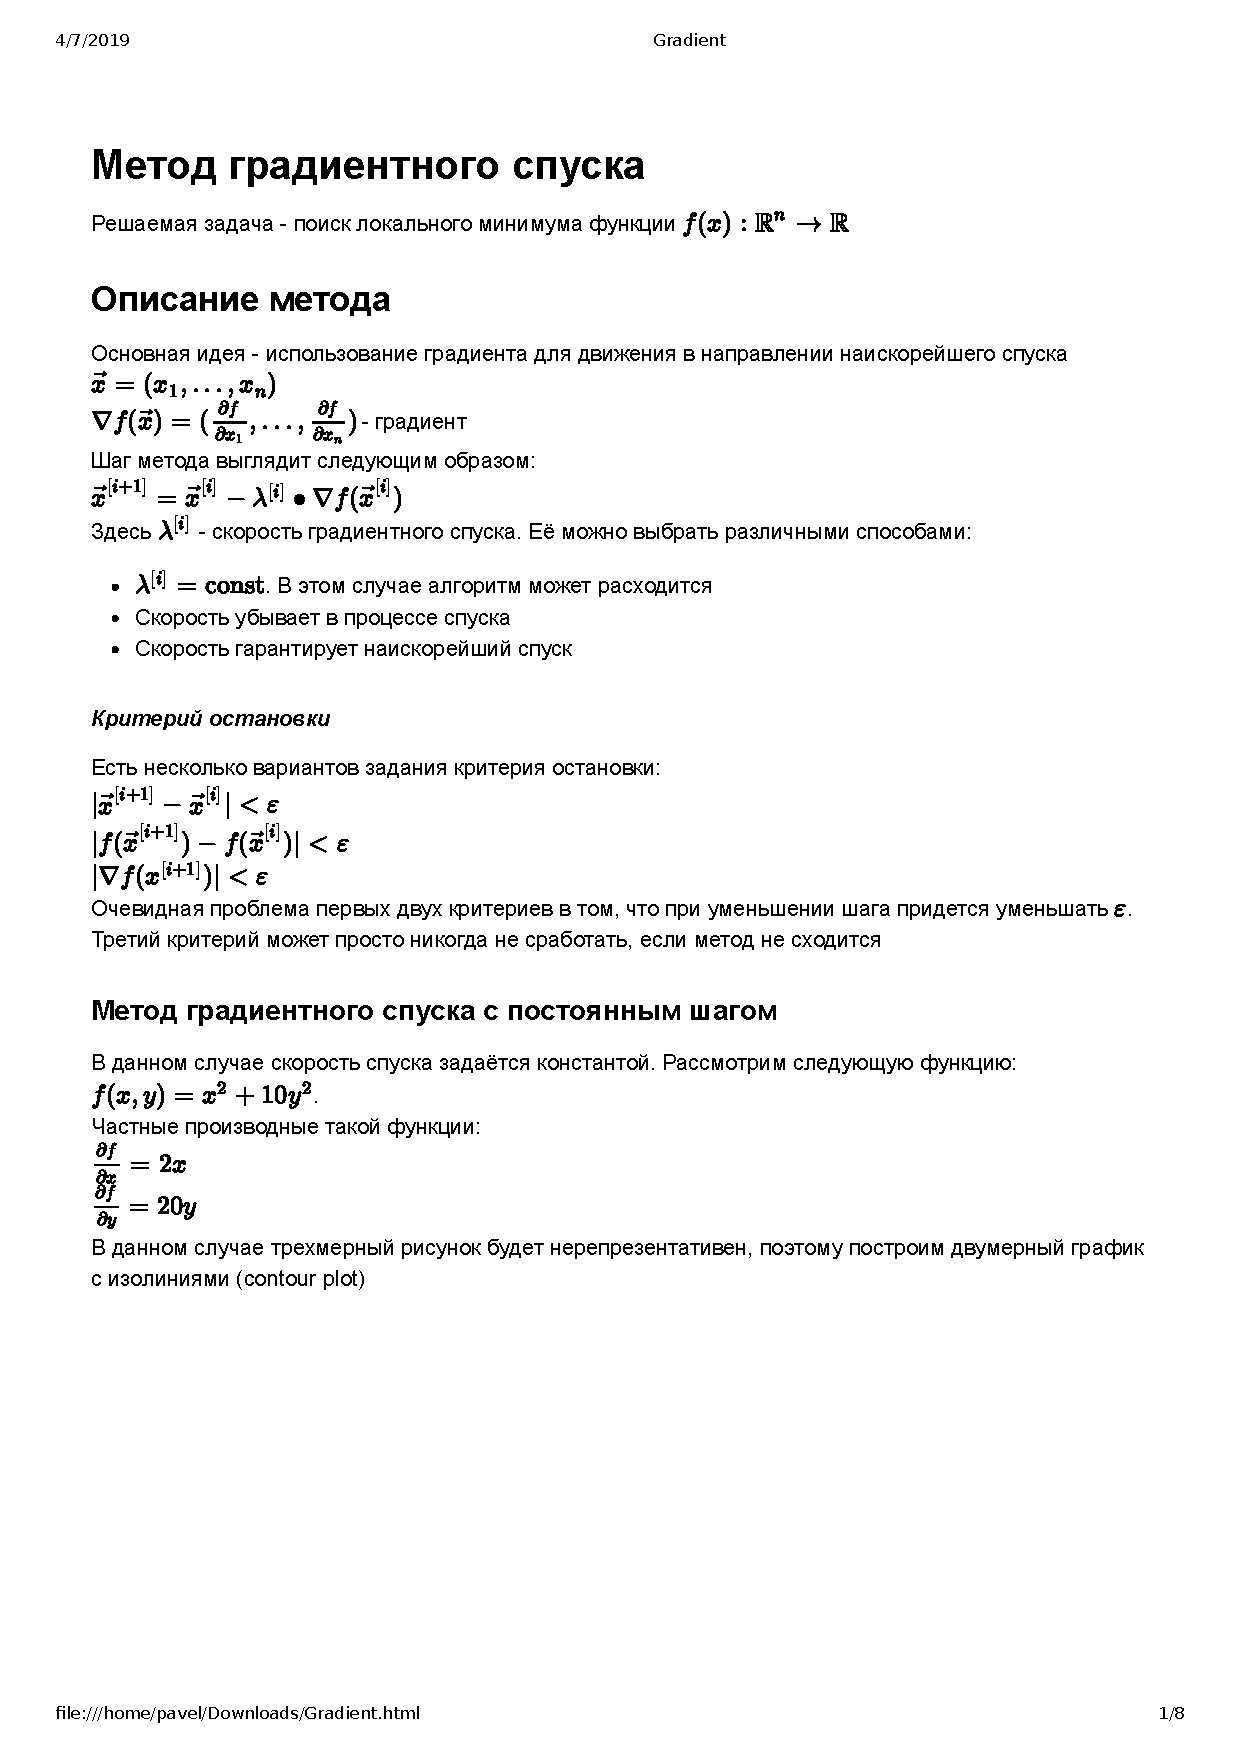
\includepdf[
	pages=-,
	addtotoc={
		1, section, 1, Приложения, suplementals,
		1, subsection, 2, ФОИТ - Метод градиентного спуска, foitgrad
	}
	]{pdf/grad.pdf}
	
	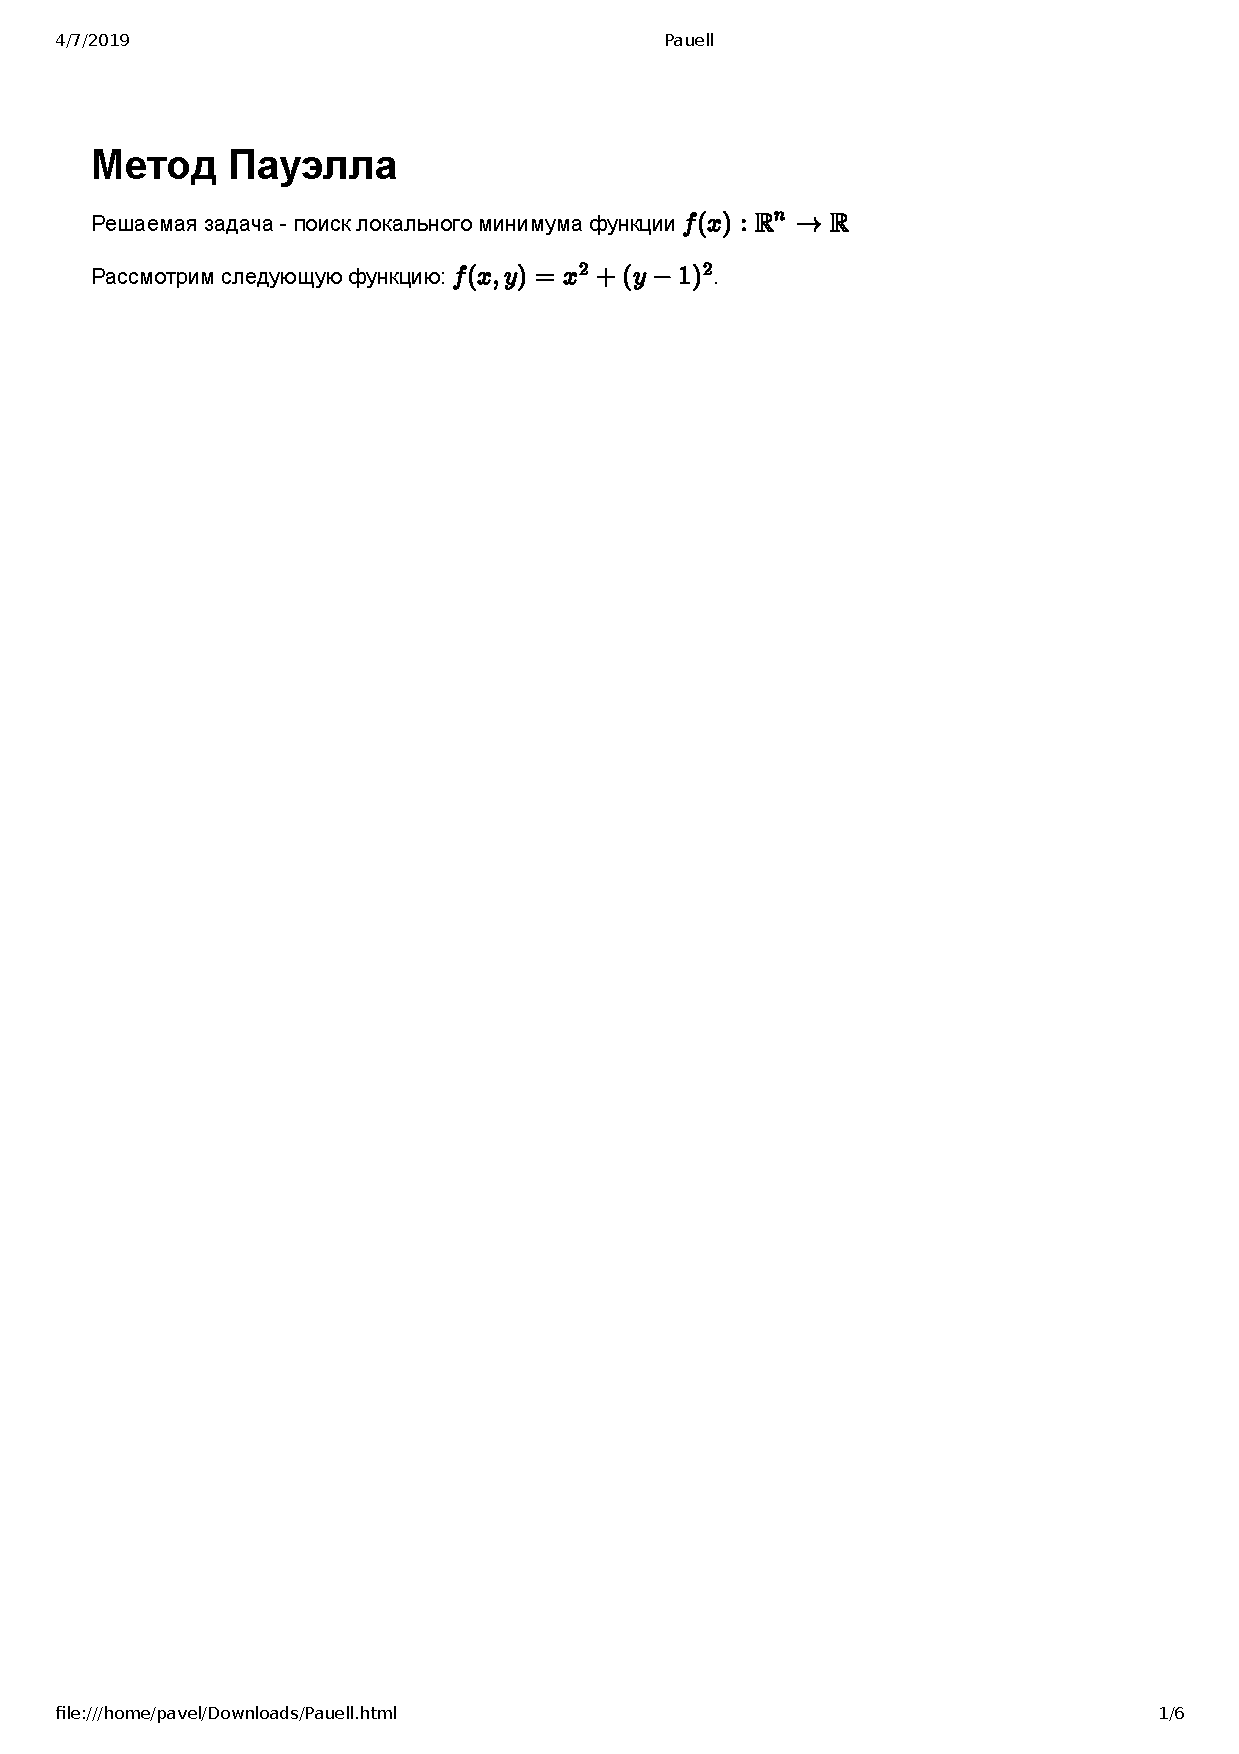
\includepdf[
	pages=-,
	addtotoc={
		1, subsection, 2, Метод Пауэлла на Python, pythonpauell
	}
	]{pdf/pauell.pdf}
	
\end{document}
